\section{Задание 2}

Сначала на странице две картинки в рамках и две кнопки с надписью ``Спрячь меня''. При нажатии на кнопку картинка прячется, и надпись на кнопке меняется на ``Покажи меня''. Если ещё раз нажать на кнопку, картинка появляется и меняется надпись на кнопке.

При нажатии на кнопку ``[Следующая картинка]'':

\begin{center}
  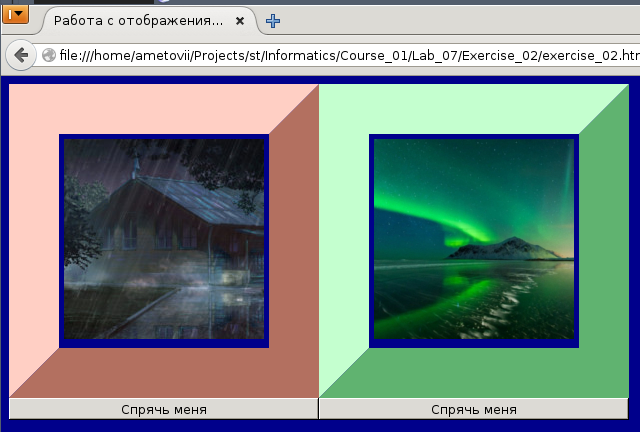
\includegraphics[width=10cm]{img/Exercise_02/01.png}
  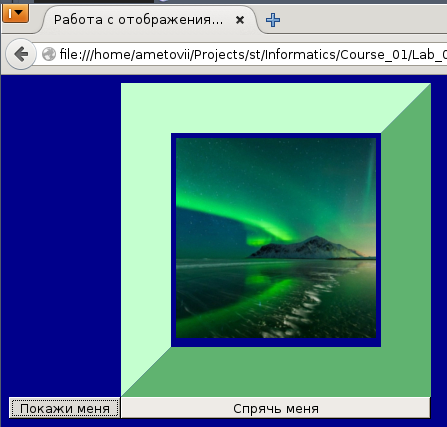
\includegraphics[width=10cm]{img/Exercise_02/02.png}
  
\includegraphics[width=10cm]{img/Exercise_02/03.png}
  
\includegraphics[width=10cm]{img/Exercise_02/04.png}
  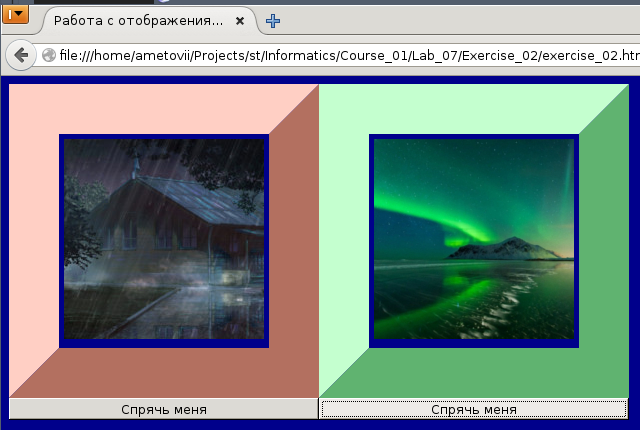
\includegraphics[width=10cm]{img/Exercise_02/05.png}
\end{center}

Исходный код \verb|exercise_02.html|:


\begin{verbatim}
<!DOCTYPE HTML>
<html>
  <head>
    <meta charset="utf-8">
    <title>Работа с отображениями картинок</title>
    <style type="text/css">
      body {
      background: darkblue;
      }
      .block1 {
          width: auto;
          height: auto;
	  float: left;
          border: outset 50px #ffA089;
      }
      
      .block2 {
          width: auto;
          height: auto;
	  float: left;
          border: outset 50px #89ffA0;
      }
    </style>
    <script>
      function changeVisibility(imageNumber){
	  var someImage=document.getElementById(imageNumber);
	  var someButton=document.getElementById('button'+
						 imageNumber);
	  if (someImage.style.display=='none'){
	      someImage.style.display='block';
	      someButton.value="Спрячь меня";
	  }
	  else {
	      someImage.style.display='none';
	      someButton.value="Покажи меня";
	  }
      }
    </script>
  </head>
  <body>
    <table cellspacing="0" cellpadding="0">
      <tr>
	<td>
	  <div class="block1" id='1'>
	    <img style="margin: 5px;" src="Pictures/01.jpeg">
	  </div>
	</td>
	<td>
	  <div class="block2" id='2'>
	    <img style="margin: 5px;" src="Pictures/02.jpg">
	  </div>
	</td>
      </tr>
      <tr>
	<td>
	  <input type="button"
		 style="width: 100%;"
		 value="Спрячь меня" id='button1'
		 onClick="changeVisibility(1)"/>
	</td>
	<td>
	  <input type="button"
		 style="width: 100%;"
		 value="Спрячь меня" id='button2'
		 onClick="changeVisibility(2)"/>
	</td>
      </tr>
    </table>
  </body>
</html>
\end{verbatim}
